% LectureTemplate for ME3050 -  Dynamics Modeling and Controls - Tennessee Technological University
% Tristan Hill - Spring 2020 - Summer 2020 - Fall 2022
% Dynamics Modeling and Controls
% Lecture Module - ODE Review - Topic 1  -

% Document settings

%\documentclass{beamer}                  % for presentation ?
\documentclass[handout]{beamer}  % for handout ?

\usepackage{../dmc_lectures} % .sty in parent folder


\newcommand{\TNUM}{1\hspace{2mm}} % Topic number 
\newcommand{\moduletitle}{ODE Review} % Titles and Stuff
\newcommand{\topictitle}{---} 

\newcommand{\sectiontitleI}{---} % More Titles and Stuff
\newcommand{\sectiontitleII}{---}
\newcommand{\sectiontitleIII}{---}
\newcommand{\sectiontitleIV}{---}

\author{ME3050 - Dynamics Modeling and Controls}
\title{Lecture Module - \moduletitle}
\date{Mechanical Engineering\vspc Tennessee Technological University}

\begin{document}

\lstset{language=MATLAB,basicstyle=\ttfamily\small,showstringspaces=false}

\frame{\titlepage \center\begin{framed}\Large \textbf{Topic \TNUM - \topictitle}\end{framed} \vspace{5mm}}

% Section 0 - Outline
\frame{
	
	\large \textbf{Topic \TNUM - \topictitle} \vspace{3mm}\\
	
	\begin{itemize}
	
		\item \sectiontitleI    \vspc % Section I
		\item \sectiontitleII 	\vspc % Section II
		\item \sectiontitleIII 	\vspc %Section III
		\item \sectiontitleIV 	\vspc %Section IV
	
	\end{itemize}

}

% Section I
\section{\sectiontitleI}

	% Section I - Frame I
	\frame{
		\frametitle{\sectiontitleI}

		We have previously derived the accepted equation of motion for this simple but fundamental system.\vspcc 		
		\begin{multicols}{2}
%		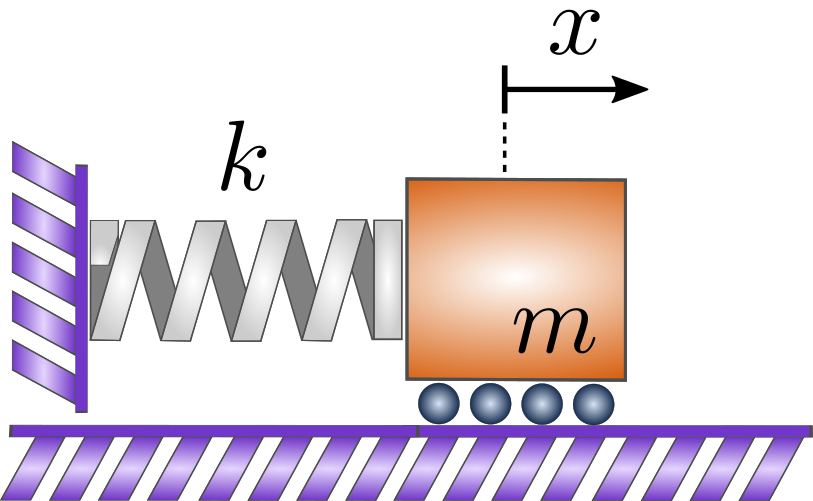
\includegraphics[scale=.20]{fancy_mass_spring.png}
		
		\[m\ddot{x}+kx=0\]
		\end{multicols}

	}
	
	% Section I - Frame II
	\frame{
		\frametitle{\sectiontitleI} \small
		
		\underline{Dynamic Simulation}	\vspc
		A simulation is an approximate imitation of the operation of a process or system;[1] that represents its operation over time. {\tiny definition \href{https://en.wikipedia.org/wiki/Simulation}{Wikipedia}} \vspc
		
		\underline{System Analysis in the Time Domain}
		\begin{framed}
			{\bf We study the motion and forces in the system as they change over time in response to various initial conditions and external forces}. \vspc
			This idea is known as the {\B time response} and we will discuss the derivations and resulting {\PN response equations} for a generalized system model as we proceed (System Dynamics, Ch. 8). \vspcc
		\end{framed}
				    
	}

% Section II
\section{\sectiontitleII}
	
	% Section II - Frame I
	\frame{
		\frametitle{\sectiontitleII}
		\small
		\begin{multicols}{2}

			Imagine you displaced the mass, and then released it from rest.
			
			\begin{framed}
				Equation of Motion:
				\[m\ddot{x}+kx=0\]
				
				Initial Position:
				\[x(t=0)=x(0)=x_0\]
				
				Initial Velocity:
				\[\dot{x}(t=0)=v(0)=v_0\]
			\end{framed}
			
			%\hspace{20mm}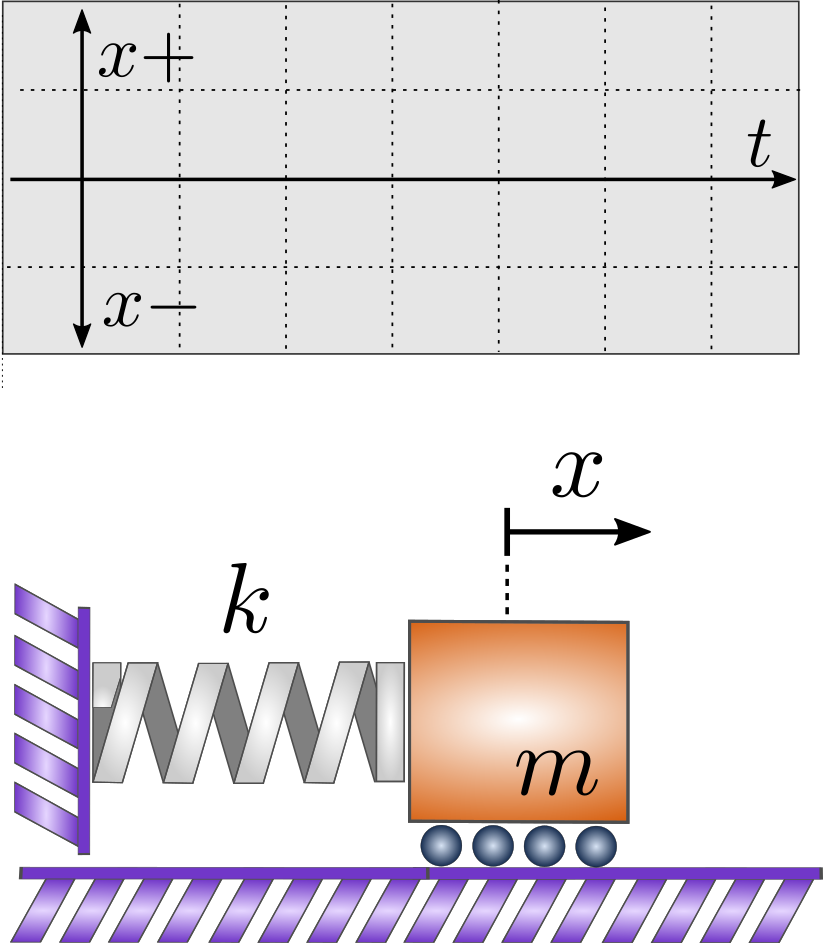
\includegraphics[scale=.20]{mass_spring_waxis.png} 
		\end{multicols}	
				
	}
		
	% Section II - Frame II
	\frame{ 
		\frametitle{\sectiontitleII}
		\small
		The {\PR free response} is found as the {\it solution the differential equation} subject to known initial conditions with zero external forced applied. \vspc
	
		\[m\ddot{x}+kx=0\hspc,\hspccc x(0)=x_0\hspc,\hspccc \dot{x}(0)=v_0\]
	
		\vspace{30mm}
			
	}

	% Section II - Frame III
	\frame{ 
		\frametitle{\sectiontitleII}
	
	
	}

% Section III
\section{\sectiontitleIII}
	
	% Section III - Frame I
	\frame{
		\frametitle{\sectiontitleIII}
	
		\[x(t)=\] 
		%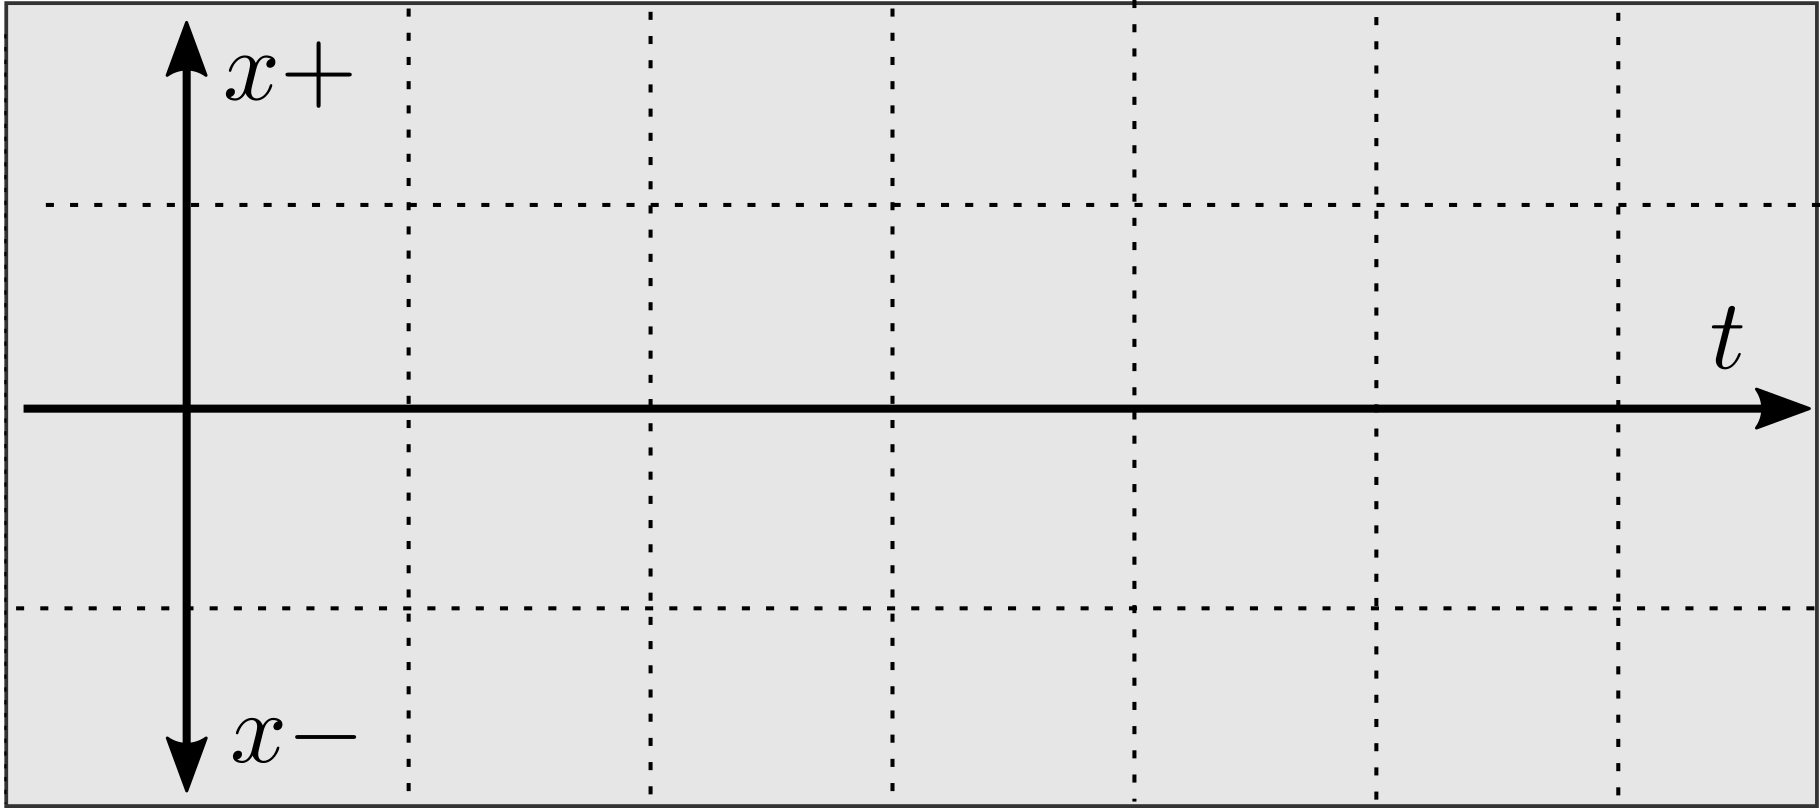
\includegraphics[scale=.2]{time_axis.png}
	}
		
% Section IV:
\section{\sectiontitleIV}

	% Section IV - Frame I
	\frame{
		\frametitle{\sectiontitleIV}
		
		Look at the system response subject to various initial conditions. What determines the amplitude and frequency of oscillation?

	}
	
\end{document}




